\documentclass[utf8x, 12pt]{G7-32} 


% --------- -------- SETTINGS --------- --------

% --------- Настройки стиля ГОСТ 7-32 --------

% Гипертекстовое оглавление в PDF
\usepackage[
bookmarks=true, colorlinks=true, unicode=true,
urlcolor=black,linkcolor=black, anchorcolor=black,
citecolor=black, menucolor=black, filecolor=black,
]{hyperref}

\usepackage{graphicx}   % Пакет для включения рисунков
\DeclareGraphicsExtensions{.jpg,.pdf,.png}
\geometry{right=20mm}
\geometry{left=30mm}
\usepackage{enumerate}
\setcounter{tocdepth}{3} % Подробность оглавления


% --------- other settings --------
\usepackage{MnSymbol}
%\usepackage{simpsons}
% --------- -------- SETTINGS --------- --------


% LISTINGS
\usepackage{listings}
\usepackage{color}

\definecolor{dkgreen}{rgb}{0,0.6,0}
\definecolor{gray}{rgb}{0.5,0.5,0.5}
\definecolor{mauve}{rgb}{0.58,0,0.82}

\lstset{frame=tb,
  language=bash,
  aboveskip=3mm,
  belowskip=3mm,
  showstringspaces=false,
  columns=flexible,
  basicstyle={\small\ttfamily},
  numbers=none,
  numberstyle=\tiny\color{gray},
  keywordstyle=\color{blue},
  commentstyle=\color{dkgreen},
  stringstyle=\color{mauve},
  breaklines=true,
  breakatwhitespace=true,
  tabsize=3
}





\begin{document}

\frontmatter 

% --------- -------- TITLE --------- --------

\begin{center} 

\large САНКТ-ПЕТЕРБУРГСИЙ ГОСУДАРСТВЕННЫЙ ПОЛИТЕХНИЧЕСКИЙ УНИВЕРСИТЕТ

\large Кафедра Компьютерных Систем и Программных Технологий \\[5.5cm] 

\huge ОТЧЕТ \\[0.6cm] % название работы, затем отступ 0,6см
\large по лабораторной работе №4\\
\large Тема: <<Утилита для исследования сети и сканер портов Nmap>>\\
\large Дисциплина: <<Методы и средства защиты информации>>\\[3.7cm]

\end{center} 

\begin{flushright}
Выполнил: студент гр. 53501/2 \\
Федоров Е.М. \\[1.2cm]


Преподаватель \\
Вылегжанина К.Д.
\end{flushright}


\vfill 

\begin{center} 
\large Санкт-Петербург \\
2015
\end{center} 

\thispagestyle{empty}


% --------- -------- TITLE --------- --------

\thispagestyle{empty}
\setcounter{page}{0}
\tableofcontents
\clearpage
\mainmatter


\chapter{Задание}

\begin{enumerate}
	\item Проверить поиск активных хостов
	\item Определить открытые порты
	\item Определить версии сервисов
	\item Изучить файлы nmap-services, nmap-os-db, nmap-service-probes
	\item Добавить новую сигнатуру службы в файл nmap-service-probes (для этого создать минимальный tcp server, добиться, чтобы при сканировании nmap указывал для него название и версию)
	\item Сохранить вывод утилиты в формате xml
	\item Исследовать различные этапы и режимы работы nmap с использованием утилиты Wireshark
\end{enumerate}


\chapter{Выполнение}


\section{Начальные настройки}

\begin{figure}[hhh!]
	\begin{center}
		
		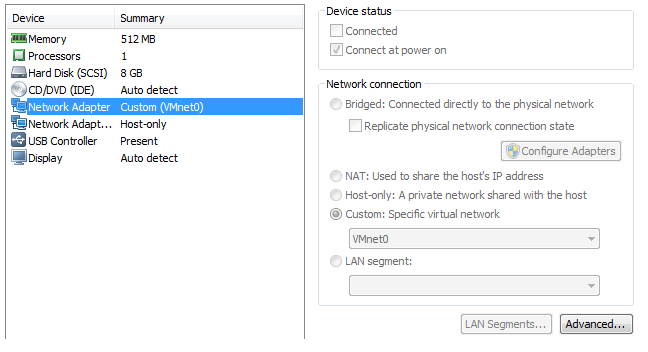
\includegraphics[width=7cm]{img2/nastr}
	\end{center}
\end{figure}




\newpage
\section{Проверить поиск активных хостов}

\begin{figure}[hhh!]
	\begin{center}
		
		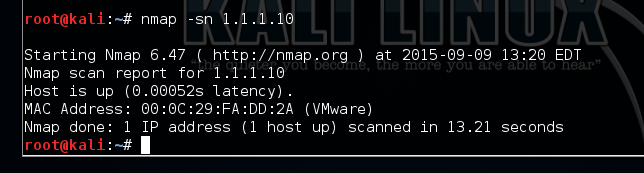
\includegraphics[width=7cm]{img2/22}
	\end{center}
\end{figure}



\newpage
\section{Определить открытые порты}

Для сканирования открытых портов предварительно запустим Metaspoit. Его адрес в сети --- 1.1.1.10. Просканируем весь диапазон его портов:

\begin{figure}[hhh!]
	\begin{center}
		
		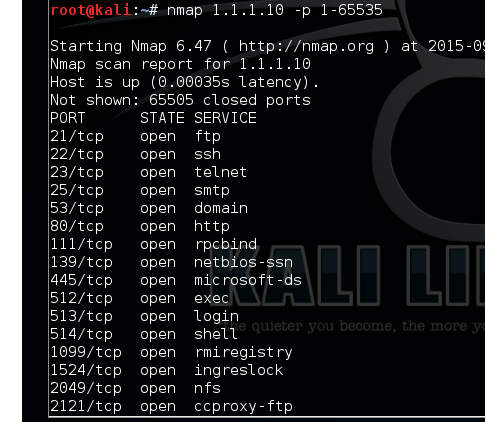
\includegraphics[width=7cm]{img2/23}
	\end{center}
\end{figure}



\newpage
\section{Определить версии сервисов}

Вновь будем сканировать Metasploit:

\begin{figure}[hhh!]
	\begin{center}
		
		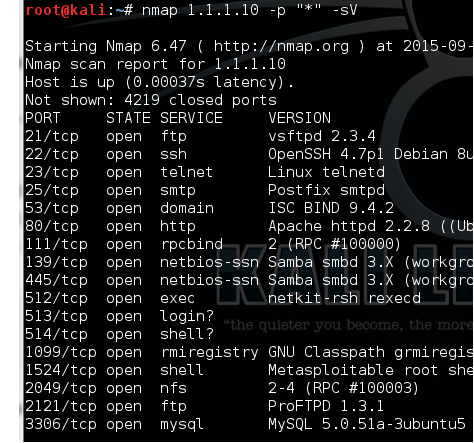
\includegraphics[width=7cm]{img2/24}
	\end{center}
\end{figure}

\newpage
\section{Изучить файлы nmap-services, nmap-os-db, nmap-service-probes}

\begin{enumerate}
	\item {\it nmap-services}\\
		Структура данного файла представлена в виде таблицы с тремя колонками:
\begin{enumerate}
	\item Имя сервиса
	\item Номер и тип порта
	\item Как часто данный порт встречается.
\end{enumerate}	

	\bigskip
Фрагмент файла:
\begin{lstlisting}
root@kali:~# cat /usr/share/nmap/nmap-services | more
# THIS FILE IS GENERATED AUTOMATICALLY FROM A MASTER - DO NOT EDIT.
...
tcpmux	1/tcp	0.001995	# TCP Port Service Multiplexer [rfc-1078]
tcpmux	1/udp	0.001236	# TCP Port Service Multiplexer
compressnet	2/tcp	0.000013	# Management Utility
...
\end{lstlisting}
	
	
	\item {\it nmap-os-db}\\
	Содержит набор отпечатков для каждой ОС представленных различными директивами.
Генерируются шесть пакетов специального вида, которые посылаются целевой машине с перерывом в 100 мс. Для получения результатов теста используются директивы:

\begin{itemize}
	\item SEQ --- результаты последовательного анализа
	\item OPS --- флаги пакетов, полученных в ответ
	\item WIN --- размер окон
	\item T1 --- данные касательно ответа на первый пакет
\end{itemize}
	\bigskip
	Также отпечаток может содержать директивы T2--T7 посылающие пакеты различного вида. Например, без указания флагов, с указанием флагов SYN, FIN, URG, PSH; а также пакеты другого вида.
	
	Кроме того, существует возможность тестировать указанный хост с помощью UDP пакетов (директива U1), а также множество других возможностей.

	Модификация данного файла достаточно сложна и, как правило, производиться крайне редко.
\begin{lstlisting}	
	root@kali:~# cat /usr/share/nmap/nmap-os-db | more
# Nmap OS Fingerprinting 2nd Generation DB. -*- mode: fundamental; -*-
...
root@kali:~# cat /usr/share/nmap/nmap-os-db | more
# Nmap OS Fingerprinting 2nd Generation DB. -*- mode: fundamental; -*-
...
\end{lstlisting}
	\item {\it nmap-service-probes}
	Основные директивы, используемые в файле.	
	\begin{itemize}
		\item Probe <протокол> <имя> q"<посылаемая строка>"\\
			Указывает nmap, какие данные отправлять в процессе определения служб
	
		\item match <название сервиса> <шаблон> [<версия>]\\
			Указывает nmap на то, как точно определить службу, используя полученный ответ на запрос.
		\item softmatch <название сервиса> <шаблон> [<версия>]\\
			Аналогичен match, но не прекращает сопоставление в случае успеха.
		\item totalwaitms <миллисекунды>\\
			Время ожидания
	\end{itemize}
\end{enumerate}

\begin{lstlisting}
root@kali:~# cat /usr/share/nmap/nmap-service-probes | more
# Nmap service detection probe list -*- mode: fundamental; -*-
...
match 1c-server m|^S\xf5\xc6\x1a{| p/1C:Enterprise business management server/
...
\end{lstlisting}

\newpage
\section{Добавить новую сигнатуру службы в файл nmap-service-probes}

Напишем простой tcp-сервер, который просто ждет подключения клиента и отправляет ему сообщение. 

\begin{lstlisting}[language=C++]
#include <sys/socket.h>
#include <netinet/in.h>
#include <stdio.h>
#include <string.h>

int main(int argc, char**argv)
{
   int listenfd;
   int connfd;
   int msgsize;

   struct    sockaddr_in servaddr;
   struct    sockaddr_in cliaddr;

   socklen_t clilen;
   pid_t     childpid;
   char      mesg[1000];

   listenfd = socket(AF_INET, SOCK_STREAM, 0);
   bzero(&servaddr, sizeof(servaddr));

   servaddr.sin_family = AF_INET;
   servaddr.sin_addr.s_addr = htonl(INADDR_ANY);            /* ADDR: ANY! */
   servaddr.sin_port = htons(2404);                         /* PORT: 2404 */
   bind(listenfd, (struct sockaddr *)&servaddr, sizeof(servaddr));

   listen(listenfd, 1024);

   for(;;)
   {
      clilen = sizeof(cliaddr);
      connfd = accept(listenfd, (struct sockaddr *)&cliaddr, &clilen);

      if ((childpid = fork()) == 0)
      {
         close (listenfd);

         for(;;)
         {
            msgsize = recvfrom(connfd, mesg, 1000, 0, (struct sockaddr *)&cliaddr, &clilen);
            if (!strncmp(mesg,"version", 7))
            {
                strcpy(mesg, "1.0.0\n");
                msgsize = strlen(mesg);
            }
            sendto(connfd, mesg, msgsize, 0, (struct sockaddr *)&cliaddr, sizeof(cliaddr));
            
         }
         
      }
      close(connfd);
   }
}
\end{lstlisting}


Впишем следующие строчки в файл nmap-service-probes:

\begin{lstlisting}
# Simple TSP server.
Probe TCP simple-tcp-server-ver q|version\r\n|
rarity 9
ports 2404
match stcps m|^1\.0\.0$| p/Simple TCP Server/ v/1.0.0-3/
\end{lstlisting}

В результате получим:


\begin{lstlisting}
root@kali:~# nmap -sV -p 2404 1.1.1.10
Starting Nmap 6.47 ( http://nmap.org ) at 2015-06-06 15:52 EDT
Nmap scan report for eth0 (1.1.1.11)
Host is up (0.00020s latency).
PORT     STATE SERVICE VERSION
2404/tcp open  stcps   Simple TCP Server 1.0.0-3
MAC Address: B8:E8:56:10:2B:BE (Apple)
\end{lstlisting}


\newpage
\section{Сохранить вывод утилиты в формате xml}

Для того, чтобы вывести данные в xml файл достаточно вызвать команду nmap с ключом -oX и указать имя файла:

\begin{lstlisting}
root@kali:~# nmap -sn -oX output.xml 1.1.1.10
\end{lstlisting}


После этого просмотрим содержимое файла:

\begin{lstlisting}[language=XML]
root@kali:~# cat output.xml 
<?xml version="1.0"?>
<!DOCTYPE nmaprun>
<?xml-stylesheet href="file:///usr/bin/../share/nmap/nmap.xsl" type="text/xsl"?>
<!-- Nmap 6.47 scan initiated Sat Jun  6 19:15:55 2015 as: nmap -sn -oX output.xml 1.1.1.10 -->
<nmaprun scanner="nmap" args="nmap -sn -oX output.xml 192.168.1.37" start="1433632555" startstr="Sat Jun  6 19:15:55 2015" version="6.47" xmloutputversion="1.04">
<verbose level="0"/>
...
\end{lstlisting}

\newpage
\section{Исследовать различные этапы и режимы работы nmap с использованием утилиты Wireshark}


Сканирование локальной сети проводится при помощи ARP запросов. Чтобы анализировать пакеты, порождаемые утилитой nmap в wireshark в фильтре напишем <<arp>>, чтобы ловить только arp пакеты, а в терминале напишем какую-нибудь nmap  команду:


\begin{figure}[hhh!]
	\begin{center}
		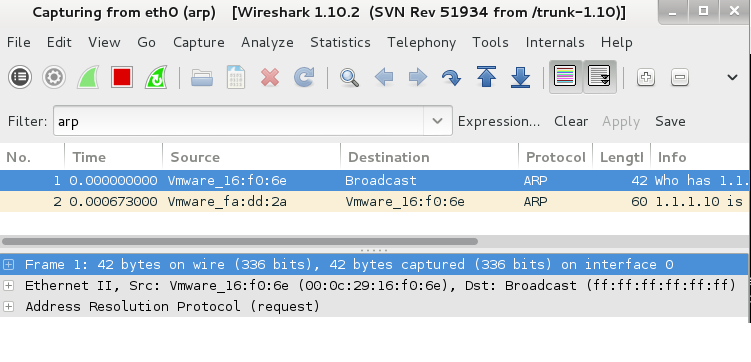
\includegraphics[width=16cm]{img2/28}
	\end{center}
\end{figure}	


 \newpage
\section{Просканировать виртуальную машину Metasploitable2 используя db nmap из состава metaspoit-framework}

Сначала включим postgresql и metasploit:

\begin{figure}[hhh!]
	\begin{center}
		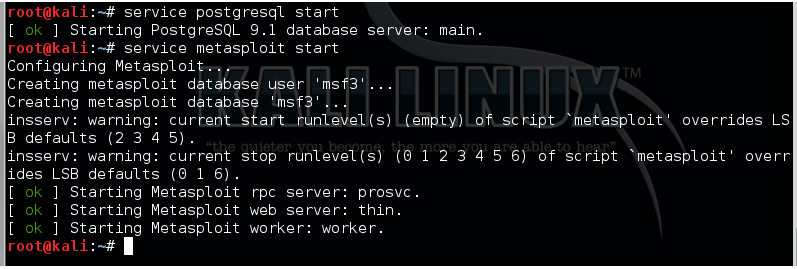
\includegraphics[width=16cm]{img2/291}
	\end{center}
\end{figure}

Перейдем в консоль metasploit framework console, будем использовать любую команду nmap, но вместо него будем использовать db nmap. Все результаты будут занесены в базу данных. Просканируем Metasploit:

\begin{figure}[hhh!]
	\begin{center}
		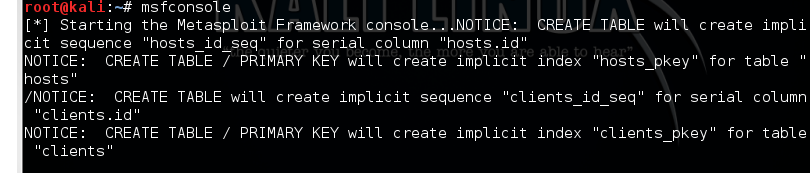
\includegraphics[width=16cm]{img2/292}
	\end{center}
\end{figure}


 \newpage
\section{Выбрать пять записей из файла nmap-service-probes и описать их работу. Выбрать один скрипт из состава Nmap и описать его работу}

\subsection{Первая запись}

\begin{lstlisting}
Probe TCP NULL q||
totalwaitms 6000
\end{lstlisting}

Запись теста с отправкой null-запроса. В данной записи будет отправляться пустой запрос по протоколу TCP. С ожиданием ответа в 6 секунд.

\subsection{Вторая запись}

\begin{lstlisting}
match 1c-server m|^S\xf5\xc6\x1a{| p/1C:Enterprise business management server/
\end{lstlisting}

 Если пользователь будет использовать nmap с ключем -sV, и после отправки
  нулевого теста с сервера приедет выражение mSxf5xc6x1a, тогда в колонке  он увидит наименование сервиса 1c-server и 1C:Enterprise business management server.


\subsection{Третья запись}
\begin{lstlisting}
Probe UDP AndroMouse q|AMSNIFF|
rarity 9
ports 8888
\end{lstlisting}

Протокол --- UDP, название --- AndroMouse, посылаемая строка --- AMSNIFF.
rarity указывает на ожидание ответа результатов от этого теста, в данном случае она очень маленькая --- 9. Взаимодействие происходит по порту 8888.

\subsection{Четвертая запись}
\begin{lstlisting}
Probe UDP FreelancerStatus q|\x00\x02\xf1\x26\x01\x26\xf0\x90\xa6\xf0\x26\x57\x4e\xac\xa0\xec\xf8\x68\xe4\x8d\x21|
rarity 9
ports 2302
\end{lstlisting}

Протокол --- UDP, название --- FreelancerStatus, посылаемая строка --- сообщение в определенной кодировке (скорее всего оно отображается по-другому).
rarity указывает на ожидание ответа результатов от этого теста, в данном случае она очень маленькая --- 9. Взаимодействие происходит по порту 8888.

\subsection{Пятая запись}

\begin{lstlisting}
# Offset  Type   Value                  Comment
# 0-1     uint16 0xBEF4                 Class: connection
# 2-3     uint16 0x0004                 Type: login reply
\end{lstlisting}

Комментарии, однострочные комментарии пишутся со знаком <<\#>> в начале строки.



\chapter{Выводы}

В ходе выполнения данной лабораторной работы были изучены основные возможности nmap, а именно, научился определять активные активные хосты, сканировать порты, определять версии сервисов. Были изучены основные файлы, используемые для определения версий сервисов. Изучена вохможность сохранения результатов в xml файл.

Кроме этого была рассмотрена версия db nmap, которая сохраняет результаты в БД. Данная возможность позволяет без использования сети в дальнейшем использовать информацию о конфигурации сети.


\end{document}
